\documentclass[]{elteikthesis}[2024/04/26]

\begin{document}
\documentlang{hungarian}

\begin{titlepage}
    \centering
    \vspace*{3cm}
    {\Huge\bfseries Mérési napló \par}
    \vspace{2cm}
    {\Large Sándor Balázs\par}
    \vspace{1cm}
    {\large 2025. április 24. \par}
    \vfill
    {
\includegraphics[width=0.2\textwidth]{images/elte_cimer_szines.eps}\par}
\end{titlepage}

\tableofcontents

\chapter{Mérési napló}

\section{A napló célja}
A mérési napló a diplomamunka melléklete ami minden a munka során elvégzett mérést és ezek eredményeit teljes terjedelmében tartalmazza.
Az adatbázis és annak építésének ismertetése, a mérések menete, az alkalmazott metrikák leírása és a modellek ismertetése a diplomamunka adott fejezében található.
Ez a dokumentum a tiszta mérési adatokat tartalmazza.
A mérések programkódjai a diplomamunka mellékletében és a projekt GitHub könyvtárában találhatóak. 

A projekt GitHub repository-ja:

\url{https://github.com/SandorBalazsHU/elte-ik-msc-thesis}

Az adatbázis elérhetősége:

\url{https://ikelte-my.sharepoint.com/:f:/g/personal/sabuaai_inf_elte_hu/ElwbJQikJ7VJqM1u5lmhhNMBq0_falCiRZTuLwoimmdrpA?e=hGFCxI}

\section{A mérési környezet és mérésmetodika}

\subsection{A mérési környezet}
A méréseket Google Colab Pro környezetben végeztem el Colab (Jupyter) notebook-ok segítségével Python nyelven CUDA gyorsítással. Az adatbázis építése az automatikus rendezés kivételével lokálisan történt python és shell szkriptek segítségével. 

\subsection{Az alkalmazott grafikus kártyák}
\begin{itemize}
  \item NVIDIA A100-SXM4-40GB
  \item NVIDIA L4 GPU
\end{itemize}
Az esetek többségében az L4 GPU-t használtam, ez óránként 2 számítási egységet használt fel, így gazdaságosabb volt. A különsen számításigényes tanításokhoz alkalmaztam az A100 GPU-t a sebessége miatt, de az 8 számítási egyéget fogyasztott óránként, így költséges volt használni. 
\note{
Az Inference time és az Epoch iterációs idő a két időérzékeny mérési eredmény, ilyenkor az alkalmazott GPU feltüntetésre kerül.
}

\subsection{Az alkalmazott szoftveres környezet}
A méréseket Google Colab Pro környezetben végeztem el Colab (Jupyter) notebook-ok segítségével Python nyelven CUDA gyorsítással. Az adatbázis építése az automatikus rendezés kivételével lokálisan történt python és shell szkriptek segítségével. 
Az elkészített mérési és adatbázis építő szoftver a mellékelt tömörített fájlban, vagy a projekt Github repository-jában található.
A szoftverek működésének ismeretése a Melléklet B: Elkészített szoftverek részben található.

\subsection{Mérésmetodika}
Az adathalmaz két osztályozása készült el:
\begin{itemize}
  \item ImageNet1k osztályozás. 114 kategória (Ezt vizsgáltam most.)
  \item Places365 osztályozás.  121 kategória (Ez a jövőbeli vizsgálatok alapja lesz.)
\end{itemize}
Az adathalmaz három részre lett felosztva:
\begin{itemize}
  \item Train 80\%: A teljes tanító adathalmaz.
  \item Val   10\%: A validációs adathalmaz a tanítshoz.
  \item Test  10\%: A teszt adahalmaz
\end{itemize}
Az adathalmaz 180750 képet tartalmaz 114 kategóriával. 
Minden mérés a ugyanazon a Test adahalmazon lett elvégezve
A mérések három lépésben kerültek lebonyolításra:
\begin{enumerate}
  \item fázis: Alapértékek meghatározása: Minden modell tanítás nélküli tesztelése ugyanazon a teszt adathalmazon.
  \item NVIDIA L4 GPU
\end{enumerate}

\chapter{Az adathalmazok elemzése}

\chapter{Az ismert modellek tesztelése}

\section{I. Mérési fázis: Modellek tesztelése tanítás nélkül}

\subsection{ResNet50 modell tanítás nélküli tesztelése}

Tartalom szöveg. Lásd a \ref{fig:resnet50}.~ábrát és a \ref{tab:resnet50}.~táblázatot.

\begin{figure}[H]
  \centering
  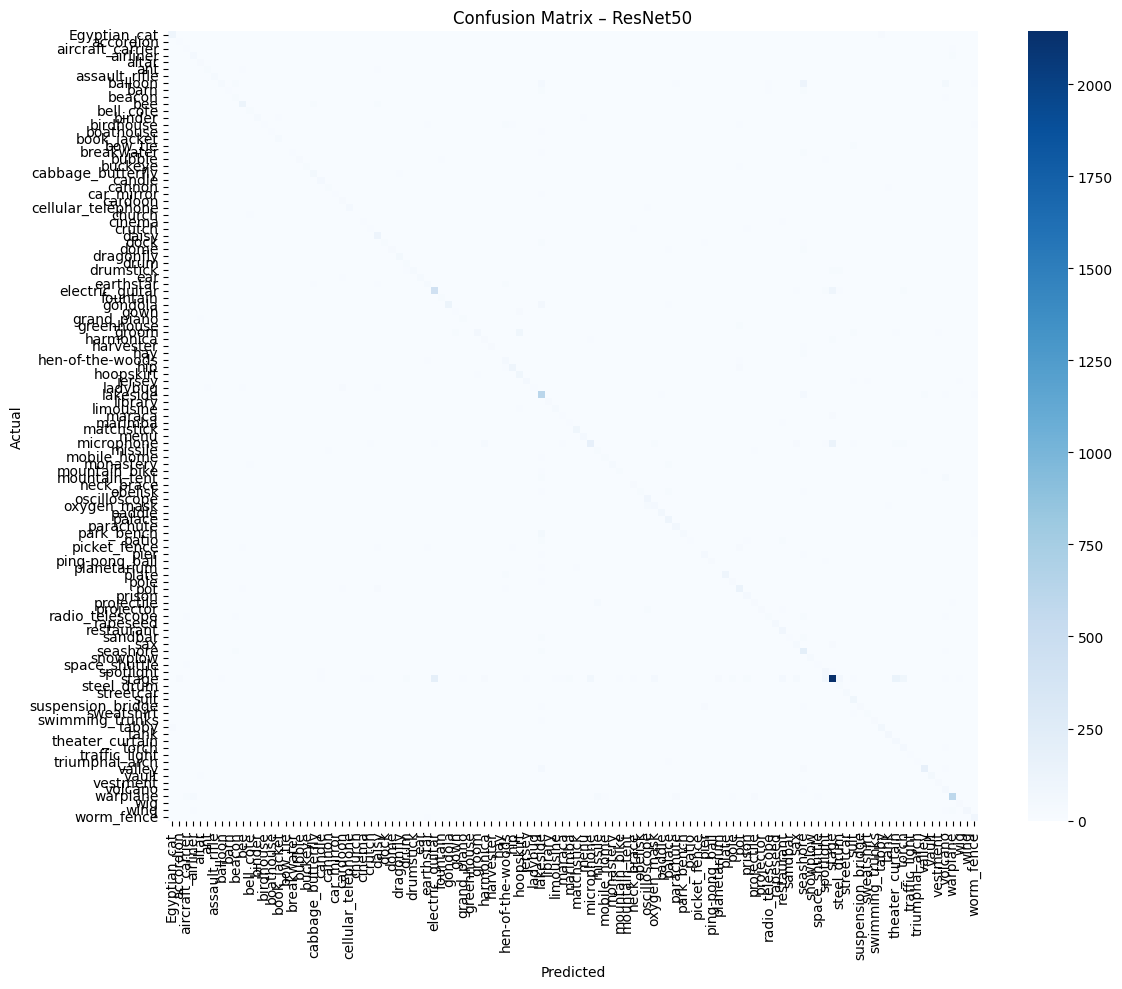
\includegraphics[width=0.9\textwidth]{images/phase01/ResNet50_basic_conf_mat.png}
  \caption{Példa ábra a ResNet50 vizsgálathoz}
  \label{fig:resnet50}
\end{figure}

\begin{table}[H]
  \centering
  \begin{tabular}{|l|c|}
    \hline
    \textbf{Metrika} & \textbf{Érték} \\
    \hline
    Top-1 Accuracy & 0.4698 \\
    Top-5 Accuracy & 0.7962 \\
    Precision & 0.3934 \\
    Recall & 0.3797 \\
    F1-score & 0.3592 \\
    Inference time & 25.21 sec \\
    \hline
  \end{tabular}
  \caption{ResNet50 @ ImageNet1k vizsgálat eredményei}
  \label{tab:resnet50}
\end{table}

\chapter{A saját modellek tesztelése}

\listoffigures
\listoftables
\end{document}